\documentclass[11pt]{article}
\usepackage{fullpage,amsthm,amsfonts,amssymb,epsfig,amsmath}
\usepackage{enumerate}
\begin{document}

\begin{center}
{\bf\large HW7 - S16}\\
Handed out 5-17 \hfill Chris Troiano \hfill 5-24, beg.
of class \\
\end{center}

\begin{enumerate}
\item 
Consider the coin changing problem:
Given an unlimited supply of coins of denominations 
$x_1, x_2,\ldots, x_n$, we wish to make change for a value $v$ using
minimum number of coins; that
is, we wish to find a smallest set of coins whose total value is $v$. 
Define a graph over the $n\times v$ grid (plus possibly some
vertices around the edges) s.t. the correct coin set corresponds to
the shortest path in this graph. 
\begin{itemize}
\item Recall the meaning of the table entries and the
recurrence.
\item Clearly describe the condition for the presence of an
  edge between two vertices of the grid.
\item How should the edges be labeled?
\item How do you find the shortest path?
\item Is this algorithm more efficient than the dynamic
  programming algorithm?
\end{itemize}
\textbf{Solution:}
Every node besides the source and sink is an entry from the coin change table.\\
An edge leaves a vertex in two possible directions: 
\begin{itemize}
\item
if we take the coin that represents the vertex we are currently observing, then an edge goes back towards the second coin we pick. The value of this edge is $v-x_i$ where $x_i$ is the current coin we are observing. 
\item
if we can't take $x_i$, then there is an edge leaving $x_i$ to the $x_{i-1}$node directly above it, the weight of this edge is $v$ because we didn't take any coins yet. Thus using the solution of the smaller coin.

\end{itemize}
\vspace*{3cm}

\item For the network given below, find the maximum flow from $S$ to
  $T$ using the Ford-Fulkerson algorithm. In each iteration
give the residual graph, the augmenting path and the
updated flow (as done in the slides). 
Also, show the corresponding minimum cut
associated with the maximum flow.\\
\textbf{Solution:}

\begin{center}
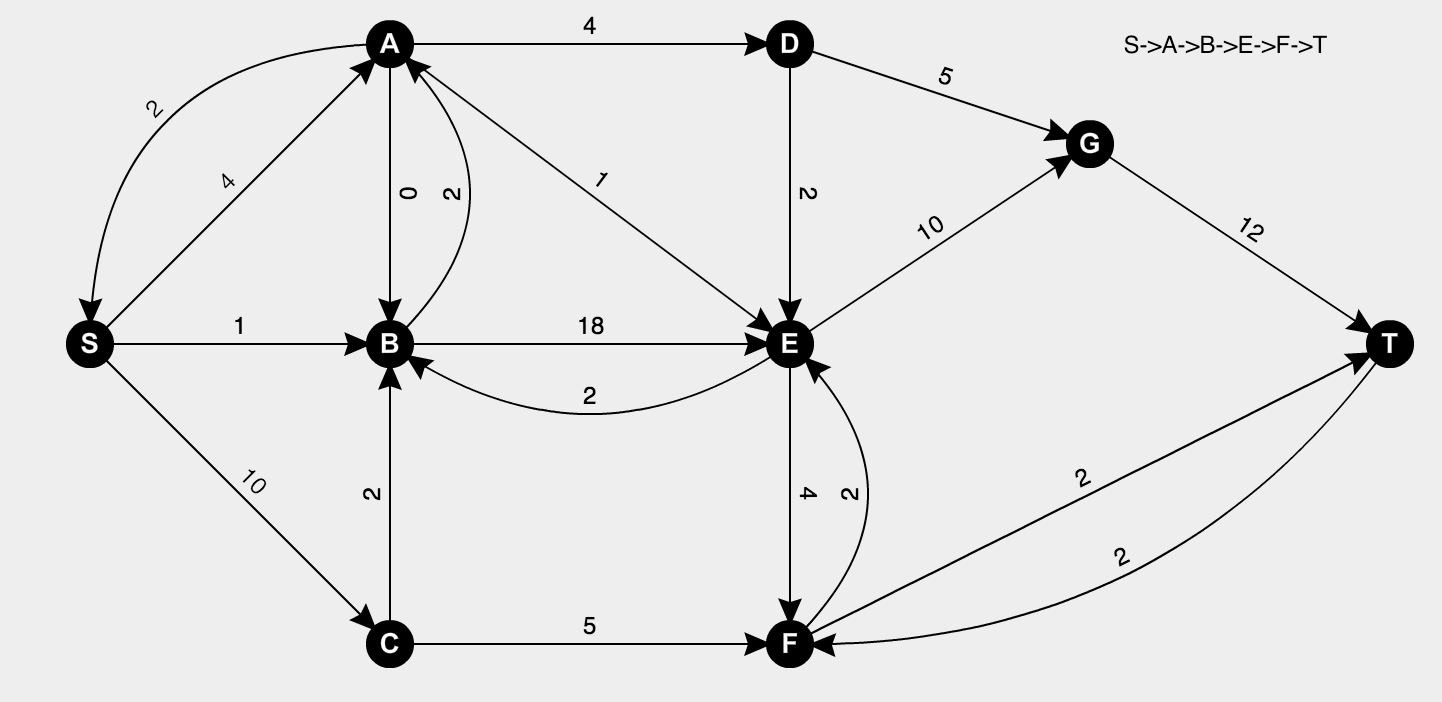
\includegraphics[scale=.4]{1st}
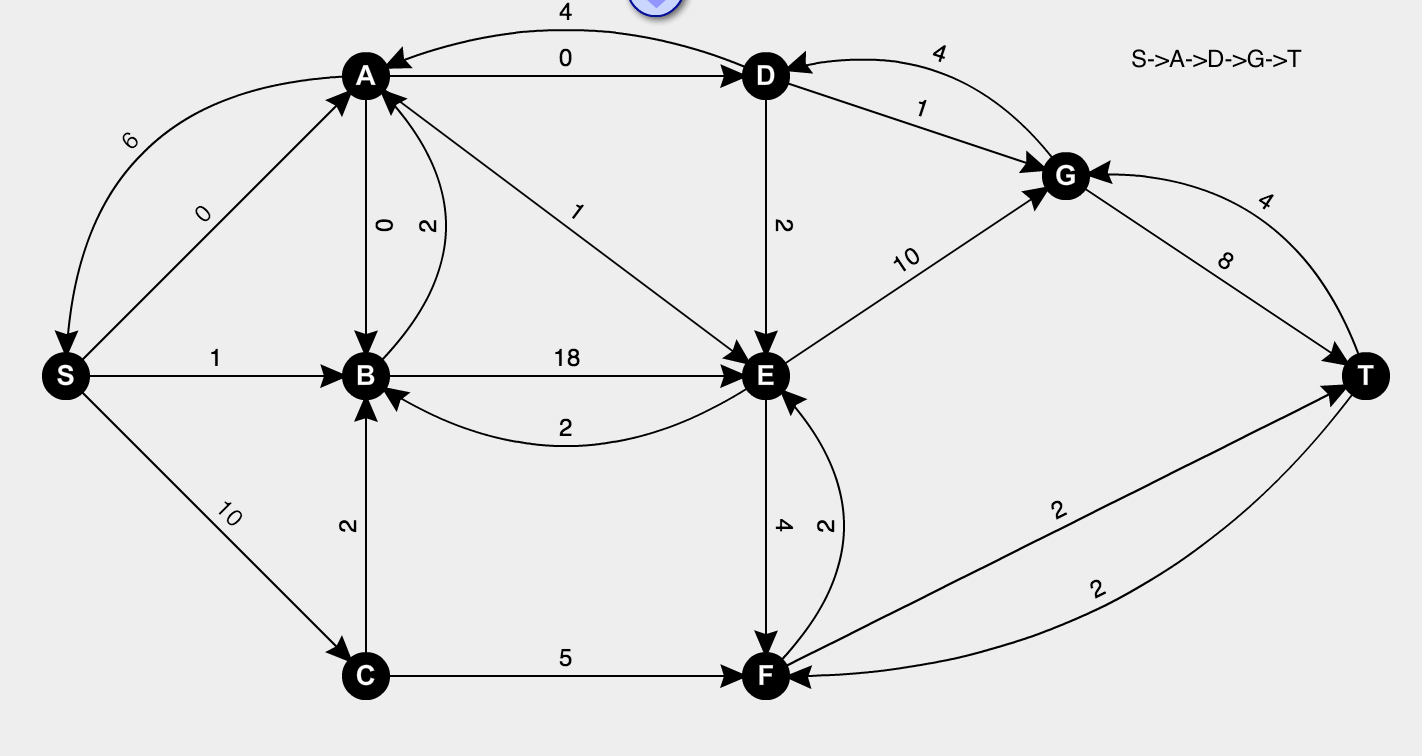
\includegraphics[scale=.4]{2nd}
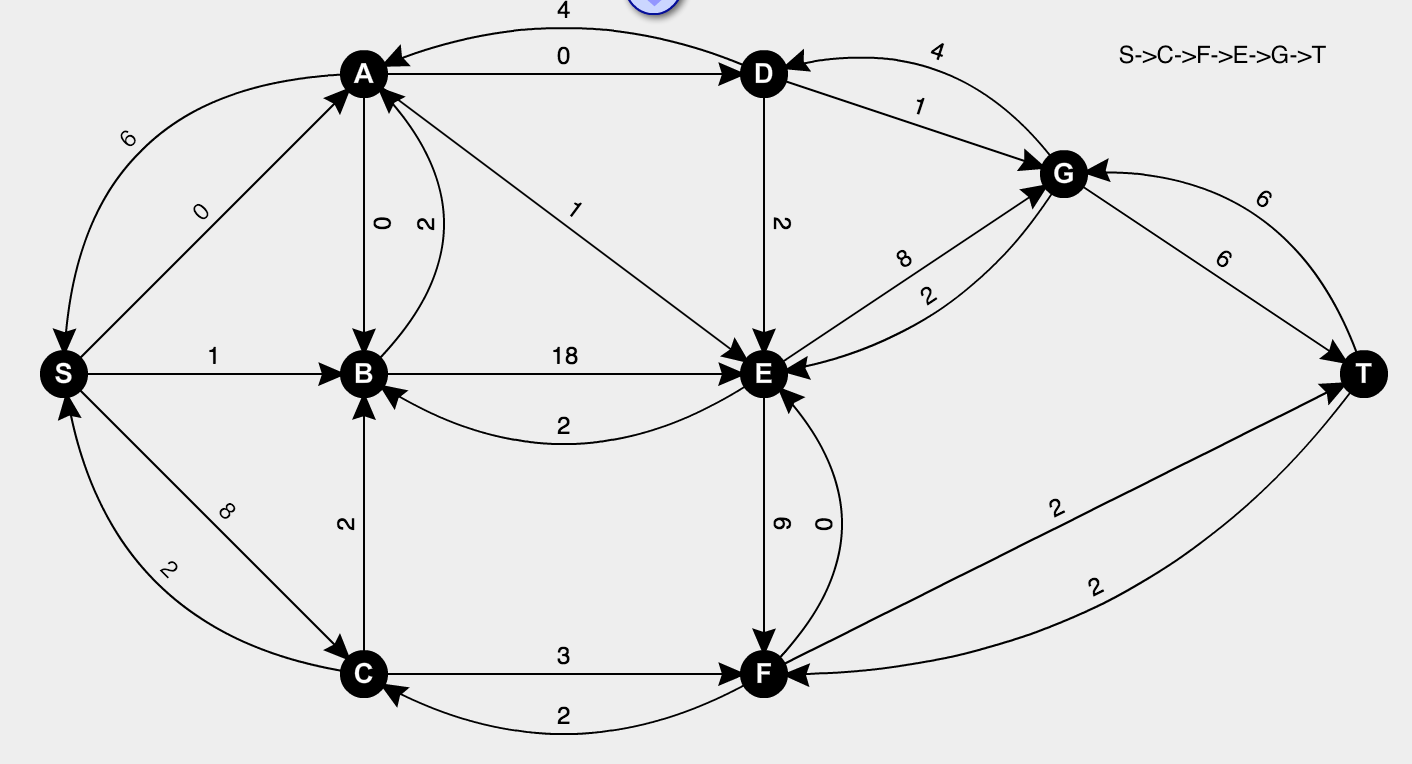
\includegraphics[scale=.4]{3rd}
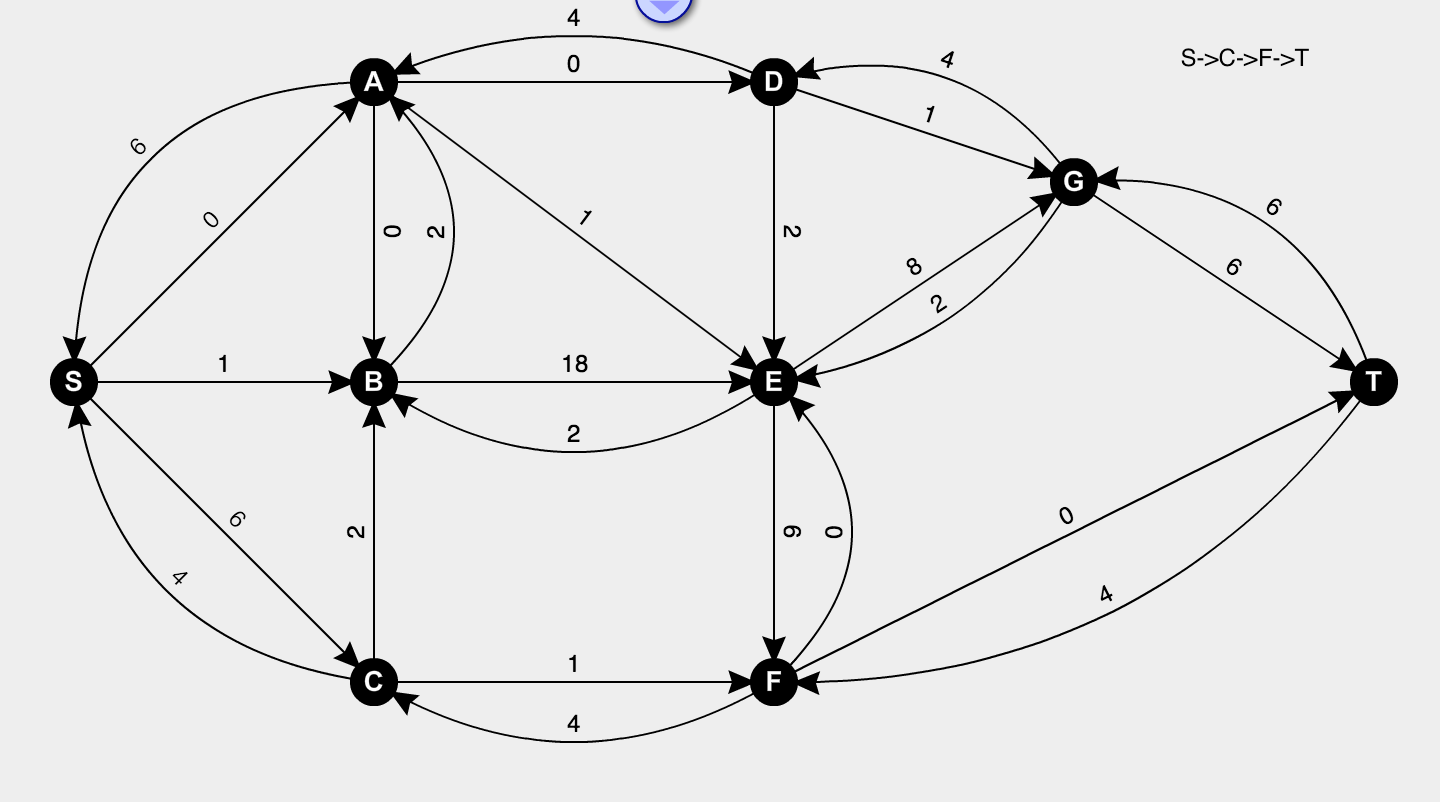
\includegraphics[scale=.4]{4th}
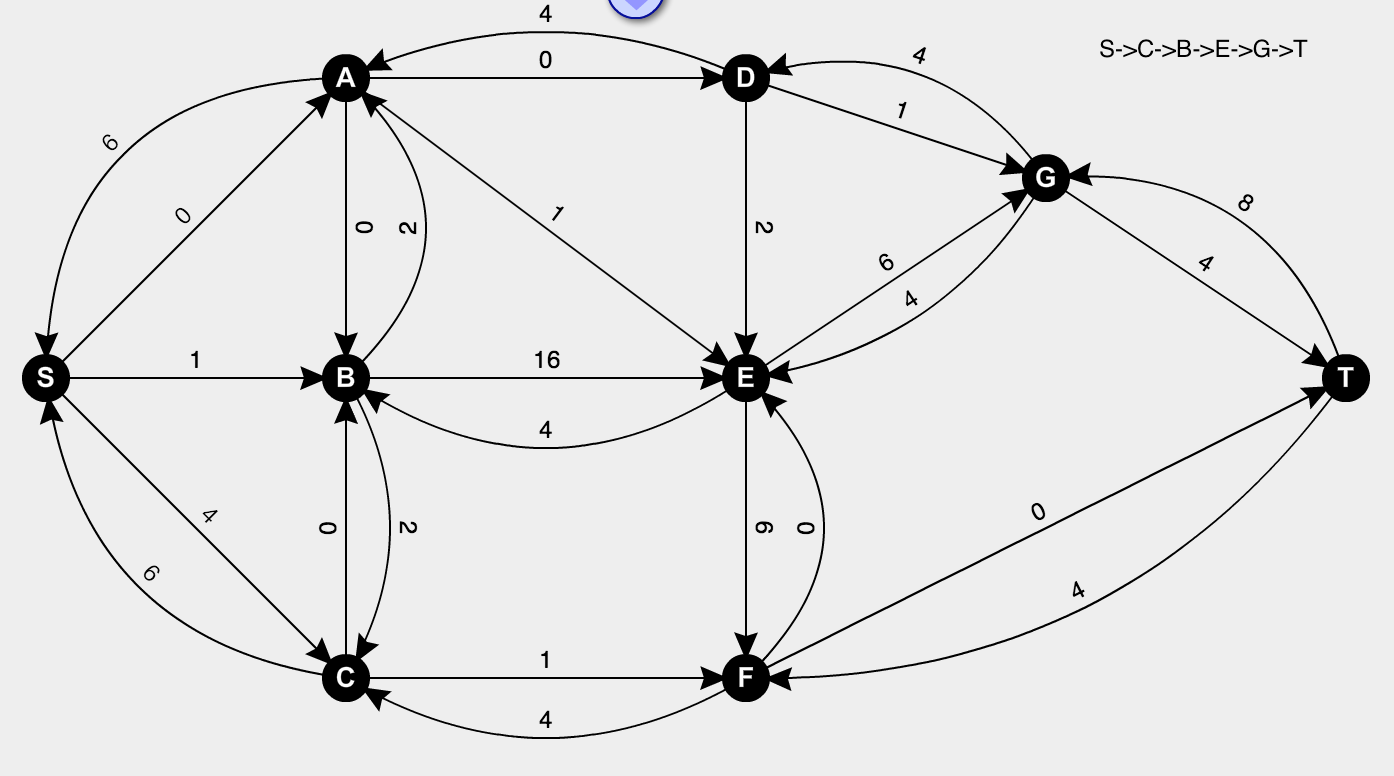
\includegraphics[scale=.4]{5th}
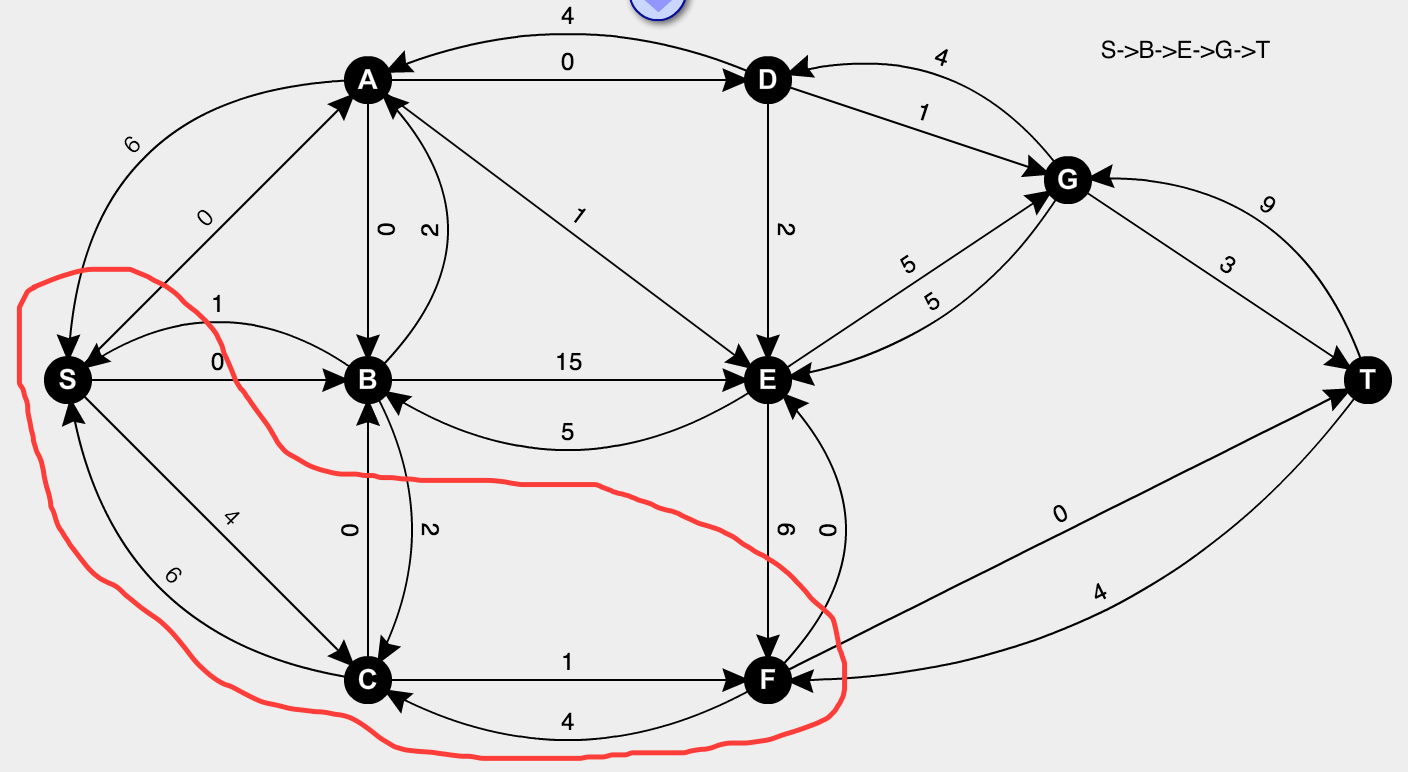
\includegraphics[scale=.4]{6th}

$min-cut: 6 + 1 + 2 + 4 = 13$ \hspace*{2cm} $max-flow: 9 + 4 = 13$
%\includegraphics[width=\textwidth]{network}
\end{center}
\item Decide whether you think the following statement is true or
  false. If it is true, give a short explanation. If it is false, give
  a counterexample.

{\em Let $G$ be an arbitrary flow network, with a source $s$, a sink
  $t$, and a positive integer capacity $c_e$ on every edge $e$ ; and
  let $(A, B)$ be a mimimum $s-t$ cut with respect to these capacities
  $\{c_e : e \in E\}$. Now suppose we add $1$ to every capacity; then
  $(A, B)$ is still a minimum $s-t$ cut with respect to these new
  capacities $\{1+c_e :e\in E\}$.}\\ 
\textbf{Solution:}\\
False, observe the two digraphs below:\\

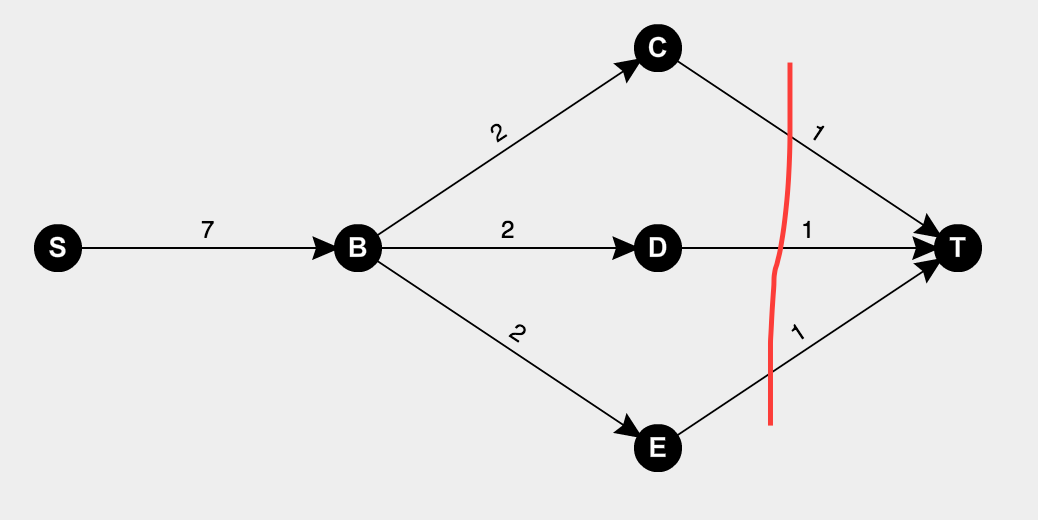
\includegraphics[scale=.4]{EX}
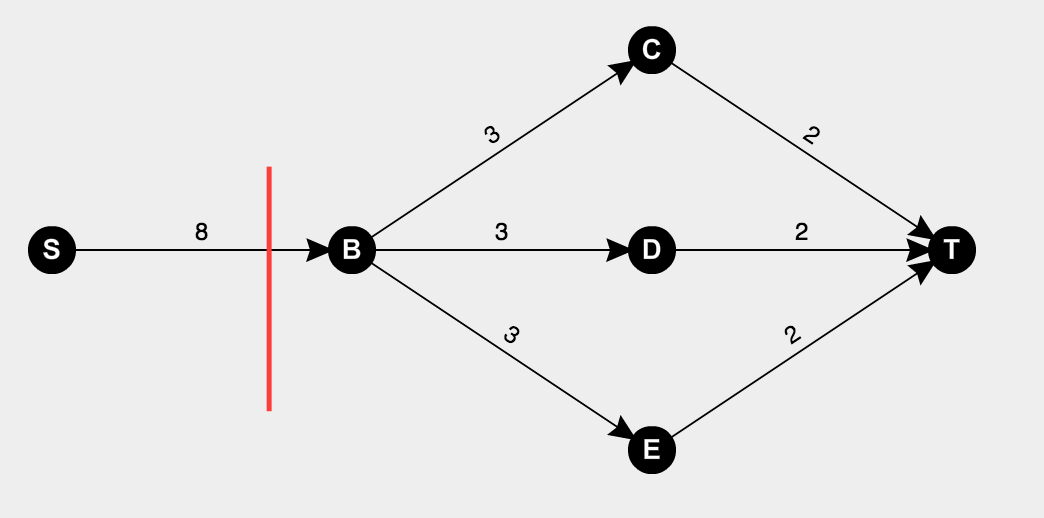
\includegraphics[scale=.4]{PLUS}



\item
There are many common variations of the maximum flow problem. Here are
two of them:
\begin{enumerate}
\item There are many sources and many sinks, and we wish to maximize the
total flow from all sources to all sinks.  
\item Each vertex also has a capacity on the maximum flow that can
  enter it.
\end{enumerate}
Both of these can be solved efficiently. Show this by reducing them to
the original max-flow problem.\\
\textbf{Solution:}\\
\begin{enumerate}
\item
To reduce this to the original max-flow problem, simply add another source and connect all of the other sources to it with infinite edges going from the new source, to the other sources. We use the same fix for the sinks. Create another sink, and connect all of the other sinks to it with infinite edges going from the other sinks to the new sink. The graph is now equivalent to an original max-flow problem.
\item
To reduce this to the original max-flow problem, we need to take each vertex and split it into two; $v_{in}$ and $v_{out}$ and then connect them by an edge that has the weight of the vertex's capacity. Then for every edge $(x, v)$ we change to $(x, v_{in})$ and $(v, y)$ we change to $(v_{out}, y)$. The graph is now equivalent to an original max-flow problem.
\end{enumerate}

\item Suppose someone presents you with a solution to a max-flow
  problem on some network. Give a linear time algorithm to determine
  whether the solution does indeed give a maximum flow. Explain the
  correctness of your algorithm. By linear time we mean
$O(n+m)$, where $n$ is the number of vertices and $m$ the
number of edges of the graph.\\
\textbf{Solution:}\\
$G'$ = run Ford-Fulkerson on $G$\\
run Dijkestra's algorithm on $G'$ from $S$ to $T$\\
\hspace*{2cm} if a result comes back, then the solution is incorrect\\
\hspace*{2cm} else, the solution is correct.\\

Correctness: After running Ford-Fulkerson, the residual graph should not allow a path from $S$ to $T$. Thus, when we run Dijkestra's and get a solution, we know that the solution we have been presented with is incorrect.\\
Time: Ford-Fulkerson's run time is $O(mf)$ where f is the weight of the heaviest edge in the graph. Dijkestra's run time is $O(m + n \log n)$. This gives us $O(n log n + 2m)$ = $O(n + m)$ time.

\end{enumerate}
\end{document}
